\section{Mapa Táctico}

En nuestro juego RTS se ha implementado un mini mapa que nos permite tener en
la esquina inferior derecha los distintos mapas de influencia y ademáas la IA táactica se
puede adaptar su comportamiento según esta influencia. En este apartado se verán los
distintos mapas implementados y su influencia táctica.

Este mapa táctico en un principio se puede ver en forma de minimapa que permite apreciar cómo varía la influencia en los distintos puntos del mapa. Esta visión táctica como ya se ha explicado se podrá alternar con el mapa de juego y así poder visualizarla en pantalla completa a la vez que cambiar el tipo de mapa táctico, mientras que el mapa de juego permanece en el minimapa.

Veamos primero cómo se ha implementado el minimapa y después entraremos más en detalle de los mapas tácticos.

\subsection{Minimapa}

Utilizando un canvas de tamaño más pequeño se ha creado un panel en la esquina inferior derecha en donde se proyectarán diferentes texturas en tiempo real. Tenemos la cámara enfocada en nuestro terreno de juego principal y otra cámara enfocada en el terreno de las influencias y las texturas en tiempo real serán las que contendrán aquello que renderice la cámara. 

Si presionamos la tecla \keys{I} podemos hacer que el mapa principal pase al mini mapa y así ver en grande los distintos mapas de influencias.  Además en esta vista tenemos un botón que nos permite cambiar entre 3 tipos de mapa: influencia, vulnerabilidad y tensión.

\begin{figure}[H]
    \centering
    \subfloat[Terreno]{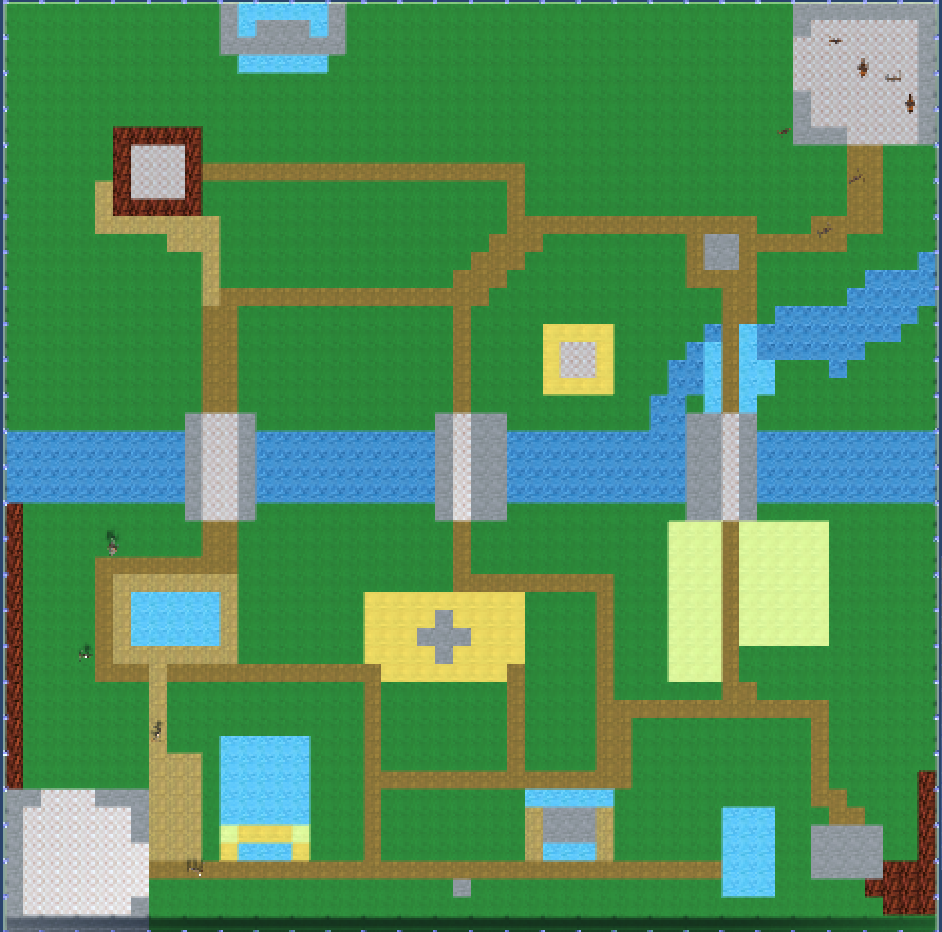
\includegraphics[width=0.2\textwidth]{images/Mapa.png}}
    \quad
    \subfloat[Influencia]{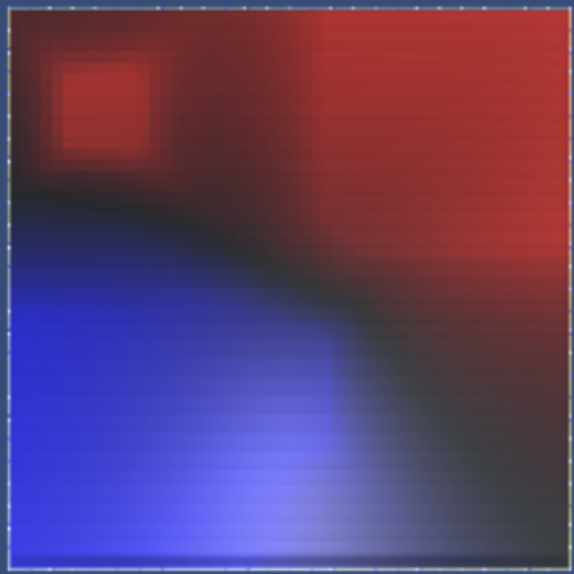
\includegraphics[width=0.2\textwidth]{images/InfluenciaMap.png}} \\
    \subfloat[Tensión]{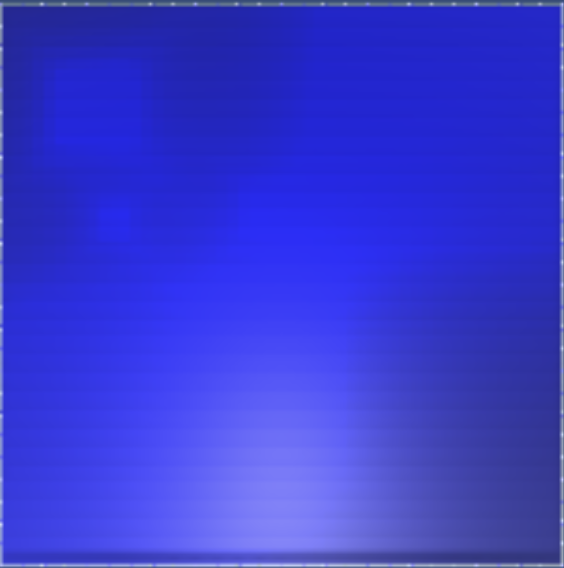
\includegraphics[width=0.2\textwidth]{images/TensionMap.png}}
    \quad
    \subfloat[Vulnerabilidad]{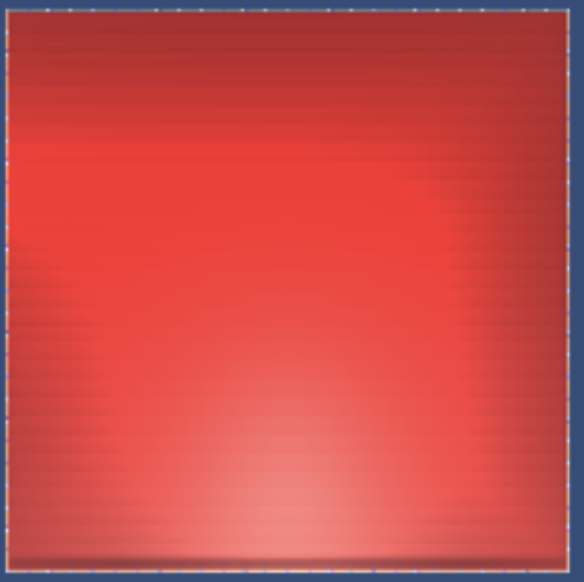
\includegraphics[width=0.2\textwidth]{images/VulnerabilidadMap.png}}
    \caption{Tipos de mapas}
\end{figure}

\subsection{Creación mapa táctico}

El mapa táctico será un grid de tamaño \qtyproduct{52 x 52}{} al igual que el mapa de juego, en este caso este tomará colores según los valores de influencia.

\subsubsection{Mapa de Influencia}

El mapa de influencia se basa en que los distintos NPCs y puntos de interés del juego tienen una influencia distintos, y estas influencias afectarán de distinta forma al comportamiento que tendrán los agentes a partir de la información que reciban de su entorno. Esta información usada por el agente puede ser el tipo de terreno, los agentes que tiene cerca, puntos de curación, etc. Este comportamiento influirá en donde se dirigen los personajes a la hora de atacar y defender. 

La influencia se calcula periódicamente y se suma a la influencia previa que hubiera en el terreno. Del mismo modo la influencia también decae pasado un cierto tiempo.

Para calcular la influencia de los distintos equipos usamos la función \texttt{UpdateTeams Influence} dentro de la clase \texttt{GridController}. Esta función obtiene la influencia previa de cada equipo (al comienzo del juego será 0), y por cada personaje y estructura perteneciente a ese equipo les asigna una influencia en su posición que posteriormente será extendida por todo el mapa.

\lstinputlisting[linerange=86-132, firstnumber=86]{\ScriptsPath/GridController.cs} 

Como se puede ver en el código para extender la influencia se hace uso de la función \texttt{ExtendInfluence}. Esta función recorre todo el terreno y asigna una influencia determinada dependiendo de la distancia. La fórmula usada para calcular como se extiende la influencia es la siguiente.
\begin{gather*}
    Influencia_{i,j} = \frac{Influencia_{base}}{1 + d\left((i,j), (x,y)\right)}
\end{gather*}
donde $i,j$ representan a la casilla dentro del terreno, $x,y$ al objeto que representa el centro de donde extiende, e $Influencia_{base}$ representa la influencia que desprende ese objeto. Por último, comentar que se utiliza la distancia de Chevychev para este cálculo.
\begin{gather*}
    d\left((i,j), (x,y)\right) = \max \left( \lvert x - i \rvert, \lvert y - j \rvert \right)
\end{gather*}

La influencia que desprende cada objeto, dependiendo de su tipo es:

\begin{table}[H]
    \centering
    \begin{tabular}{|c|c|}
        \hline
        Jugador & 0.75 \\
        \hline
        Estructura & 0.25 \\
        \hline
        NPC & 0.5 \\
        \hline
    \end{tabular}
    \caption{Influencia por tipo de objeto}
    \label{tab:influencepertype}
\end{table}

El mapa de influencia se representará como un mapa de calor con los colores rojo y azul, donde el rojo representa influencia máxima del equipo B y el azul del A. La influencia mostrada en el mapa se calculará de la siguiente forma.
\begin{gather*}
    Influencia = Influencia_A - Influencia_B
\end{gather*}
donde $Influencia_A, Influencia_B \in [0,1]$ y, por tanto, $Influencia \in [-1, 1]$.

% Cómo se calcula la influencia.

Esta información de influencias será usada como información táctica a la hora de calcular el comportamiento táctico de los personajes

\subsubsection{Mapas de Tensión y Vulnerabilidad}

Estos mapas se calculan a través de los valores de influencia de los distintos equipos y aportan información visual sobre el estado de la partida actual.

\begin{gather*}
    Tension = \frac{Influencia_A + Influencia_B}{2}
\end{gather*}
donde $Influencia_A, Influencia_B \in [0,1]$ y, por tanto, $Tension \in [0, 1]$.

\begin{gather*}
    Vulnerabilidad = Tension - \lvert Influencia \rvert
\end{gather*}
donde $Tension, \lvert Influencia \rvert \in [0,1]$ y, por tanto, $Vulnerabilidad \in [-1, 1]$.

%\subsection{Aplicación y uso de la información táctica en el comportamiento de NPCs}

